\documentclass[a4paper, 10pt, ]{article}

\usepackage[slovak]{babel}


\usepackage[utf8]{inputenc}
\usepackage[T1]{fontenc}

\usepackage[left=4cm,
			right=4cm,
			top=2.1cm,
			bottom=2.6cm,
			footskip=7.5mm,
			marginparwidth=3.0cm,
			]{geometry}

\usepackage{graphicx}
\usepackage[dvipsnames]{xcolor}
% https://en.wikibooks.org/wiki/LaTeX/Colors


% ------------------------------

\usepackage{lmodern}

\usepackage[tt={oldstyle=false,proportional=true,monowidth}]{cfr-lm}

% ------------------------------

\usepackage{amsmath}
\usepackage{amssymb}
\usepackage{amsthm}

\usepackage{booktabs}
\usepackage{multirow}
\usepackage{array}
\usepackage{dcolumn}


\usepackage[singlelinecheck=true]{subfig}

% ------------------------------

\hyphenpenalty=6000
\tolerance=1000



\def\naT{\mathsf{T}}

% ------------------------------
\makeatletter

	\def\@seccntformat#1{\protect\makebox[0pt][r]{\csname the#1\endcsname\hspace{4mm}}}

	\def\cleardoublepage{\clearpage\if@twoside \ifodd\c@page\else
	\hbox{}
	\vspace*{\fill}
	\begin{center}
	\phantom{}
	\end{center}
	\vspace{\fill}
	\thispagestyle{empty}
	\newpage
	\if@twocolumn\hbox{}\newpage\fi\fi\fi}

	\newcommand\figcaption{\def\@captype{figure}\caption}
	\newcommand\tabcaption{\def\@captype{table}\caption}

\makeatother

% ------------------------------

\usepackage{fancyhdr}
\fancypagestyle{plain}{%
\fancyhf{} % clear all header and footer fields
\fancyfoot[C]{\sffamily {\bfseries \thepage}\ | {\scriptsize\oznacenieCasti}}
\renewcommand{\headrulewidth}{0pt}
\renewcommand{\footrulewidth}{0pt}}
\pagestyle{plain}


% ------------------------------

\usepackage{titlesec}
\titleformat{\paragraph}[hang]{\sffamily  \bfseries}{}{0pt}{}
\titlespacing*{\paragraph}{0mm}{3mm}{1mm}
\titlespacing*{\subparagraph}{0mm}{3mm}{1mm}

\titleformat*{\section}{\sffamily\Large\bfseries}
\titleformat*{\subsection}{\sffamily\large\bfseries}
\titleformat*{\subsubsection}{\sffamily\normalsize\bfseries}






% ------------------------------

\PassOptionsToPackage{hyphens}{url}
\usepackage[pdfauthor={},
			pdftitle={},
			pdfsubject={},
			pdfkeywords={},
			% hidelinks,
			colorlinks=false,
			breaklinks,
			]{hyperref}


% ------------------------------

\graphicspath{%
{../FIG/}%
{../SVG/}%
{../PY/fig/}%
{../PY/jupynotex/fig/}%
{../ML/fig/}%
}



% ------------------------------

\usepackage{enumitem}

\usepackage{lettrine}

% ------------------------------

\usepackage{microtype}

% ------------------------------

\usepackage[titles]{tocloft}

\setlength{\cftsecindent}{-12mm}
\setlength{\cftsecnumwidth}{12mm}
\renewcommand{\cftsecpresnum}{\hfill}
\renewcommand{\cftsecaftersnum}{\hspace{4mm}}

\setlength{\cftsubsecindent}{-12mm}
\setlength{\cftsubsecnumwidth}{16mm} % 12 + 4
\renewcommand{\cftsubsecpresnum}{\hfill}
\renewcommand{\cftsubsecaftersnum}{\hspace{8mm}} % 4 + 4 mm

\setlength{\cftsubsubsecindent}{-12mm}
\setlength{\cftsubsubsecnumwidth}{20mm} % 12 + 4 + 4
\renewcommand{\cftsubsubsecpresnum}{\hfill}
\renewcommand{\cftsubsubsecaftersnum}{\hspace{12mm}} % 4 + 4 + 4 mm

\renewcommand{\cftsecpagefont}{\lstyle \bfseries}
\renewcommand{\cftsubsecpagefont}{\lstyle}
\renewcommand{\cftsubsubsecpagefont}{\lstyle}

\setlength{\cftparaindent}{-16mm}
\setlength{\cftparanumwidth}{28mm} % 16 + 4 + 4 + 4
\renewcommand{\cftparapresnum}{\hfill}
\renewcommand{\cftparaaftersnum}{\hspace{16mm}} % 4 + 4 + 4 + 4 mm








% ------------------------------

\usepackage{listings}

\renewcommand{\lstlistingname}{Výpis kódu}
\renewcommand{\lstlistlistingname}{Výpisy kódu}


%New colors defined below
\definecolor{codegreen}{rgb}{0,0.6,0}
\definecolor{codegray}{rgb}{0.5,0.5,0.5}
\definecolor{codepurple}{rgb}{0.58,0,0.82}
\definecolor{backcolour}{rgb}{0.95,0.95,0.95}

%Code listing style named "mystyle"
\lstdefinestyle{mystyle}{
  backgroundcolor=\color{backcolour},
  commentstyle=\fontfamily{lmtt}\fontsize{8.5pt}{8.75pt}\selectfont\color{codegreen},
  keywordstyle=\fontfamily{lmtt}\fontsize{8.5pt}{8.75pt}\selectfont\bfseries\color{Blue},
  stringstyle=\fontfamily{lmtt}\fontsize{8.5pt}{8.75pt}\selectfont\color{codepurple},
  basicstyle=\fontfamily{lmtt}\fontsize{8.5pt}{8.75pt}\selectfont,
  breakatwhitespace=false,
  breaklines=true,
  captionpos=t,
  keepspaces=true,
  numbers=left,
  numbersep=4mm,
  numberstyle=\fontfamily{lmtt}\fontsize{8.5pt}{8.75pt}\selectfont\color{lightgray},
  showspaces=false,
  showstringspaces=false,
  showtabs=false,
  tabsize=2,
  % xleftmargin=10pt,
  framesep=10pt,
  language=Python,
  escapechar=|,
}


\lstset{
    inputencoding=utf8,
    extendedchars=true,
    literate=%
    {á}{{\'a}}1
    {č}{{\v{c}}}1
    {ď}{{\v{d}}}1
    {é}{{\'e}}1
    {ě}{{\v{e}}}1
    {í}{{\'i}}1
    {ň}{{\v{n}}}1
    {ó}{{\'o}}1
    {ř}{{\v{r}}}1
    {š}{{\v{s}}}1
    {ť}{{\v{t}}}1
    {ú}{{\'u}}1
    {ů}{{\r{u}}}1
    {ý}{{\'y}}1
    {ž}{{\v{z}}}1
    {Á}{{\'A}}1
    {Č}{{\v{C}}}1
    {Ď}{{\v{D}}}1
    {É}{{\'E}}1
    {Ě}{{\v{E}}}1
    {Í}{{\'I}}1
    {Ň}{{\v{N}}}1
    {Ó}{{\'O}}1
    {Ř}{{\v{R}}}1
    {Š}{{\v{S}}}1
    {Ť}{{\v{T}}}1
    {Ú}{{\'U}}1
    {Ů}{{\r{U}}}1
    {Ý}{{\'Y}}1
    {Ž}{{\v{Z}}}1
    {ô}{{\^{o}}}1
}


% ------------------------------


\usepackage{caption}

\DeclareCaptionFormat{odsadene}{\protect\makebox[0pt][r]{#1#2\hspace{4mm}}#3\par}
\DeclareCaptionLabelSeparator{lendvojbodka}{:}
\DeclareCaptionFont{lightgray}{\fontfamily{lmtt}\fontsize{8.5pt}{8.75pt}\selectfont\color{lightgray}}

\captionsetup[lstlisting]{format=odsadene, labelsep=lendvojbodka, justification=raggedright, singlelinecheck=false, labelfont={sf, lightgray},}


% ------------------------------





% ------------------------------

\usepackage[backend=biber,
            style=numeric,
            sorting=none,
            ]{biblatex}
\DeclareSourcemap{
    \maps[datatype=bibtex]{
        \map{
        \step[fieldset=note, null]
        }
        \map{
        \step[fieldset=file, null]
        }        
        % \map{
        % \step[fieldset=url, null]        
        % }
        \map{
        \step[fieldset=eprint, null]
        }
    }
}


\addbibresource{E:/_CurrentContent/01_work_repo/bibLaTeXDB/bibLaTeXDB.bib} % nonpublic data





\def\oznacenieCasti{MRS96 - ZS2026}






\begin{document}

\lstset{style=mystyle}


\fontsize{12pt}{22pt}\selectfont

\centerline{\textsf{Modelovanie a riadenie systémov} \hfill \textsf{\oznacenieCasti}}

\fontsize{18pt}{22pt}\selectfont

\begin{flushleft}
	\textbf{\textsf{Príklady prevodových charakteristík vybraných laboratórnych zariadení}}
\end{flushleft}

\fontsize{12pt}{14pt}\selectfont




\normalsize

\bigskip

{\hypersetup{hidelinks}

\tableofcontents

}

\bigskip

\vspace{18pt}



\noindent
\lettrine[lines=3, nindent=0pt]{C}{ieľom} textu je prehľad vybraných príkladov meraní prevodových charakteristík na reálnych laboratórnych zariadeniach.






\section{O prevodovej charakteristike zariadenia LMOT}

\subsection{Opis zariadenia}


\begin{figure}[!b]
% \begin{center}

    \vbox{%


        \makebox[\textwidth][c]{%
        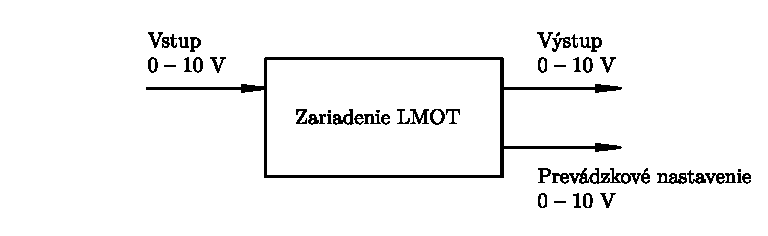
\includegraphics{LMOT_sch1.pdf}
        }

        \figcaption{ 
            Signály systému LMOT.
        }
        \label{LMOT_sch1}
    }%vbox

% \end{center}
\end{figure}


LMOT je laboratórne zariadenie predstavujúce reálny dynamický systém. Skladá sa z~jednosmerného motora, tachodynama na spoločnom hriadeli a elektronických obvodov zabezpečujúcich jeho napájanie. Elektronické obvody určujú dominantné statické a dynamické vlastnosti systému, ktoré je možné do určitej miery meniť pomocou potenciometra.

Systém má jeden vstup a jeden výstup. Vstup ovláda napájanie motora a výstupný signál je úmerný jeho uhlovej rýchlosti, snímanej tachodynamom. Poloha potenciometra určuje prevádzkové nastavenie systému a poskytuje informáciu o jeho aktuálnych vlastnostiach.

\begin{center}

\vspace{-10pt}   

\vbox{%
    
\tabcaption{Rozsahy a jednotky signálov zariadenia LMOT.}
\label{tab:rozsahy_a_jednotky_signalu}

\lstyle

\begin{tabular*}{\textwidth}{@{ \extracolsep{\fill}} lll}
\toprule
Signál & Rozsah hodnôt & Jednotka \\
\midrule
Vstup & $0$ až $10$ & V (volt) \\
Výstup & $0$ až $10$ & V (volt) \\
Prevádzkové nastavenie & $0$ až $10$ & V (volt) \\
\bottomrule
\end{tabular*}

}

\end{center}






\begin{figure}[!t]
\vbox{%

    \makebox[\textwidth][c]{%
    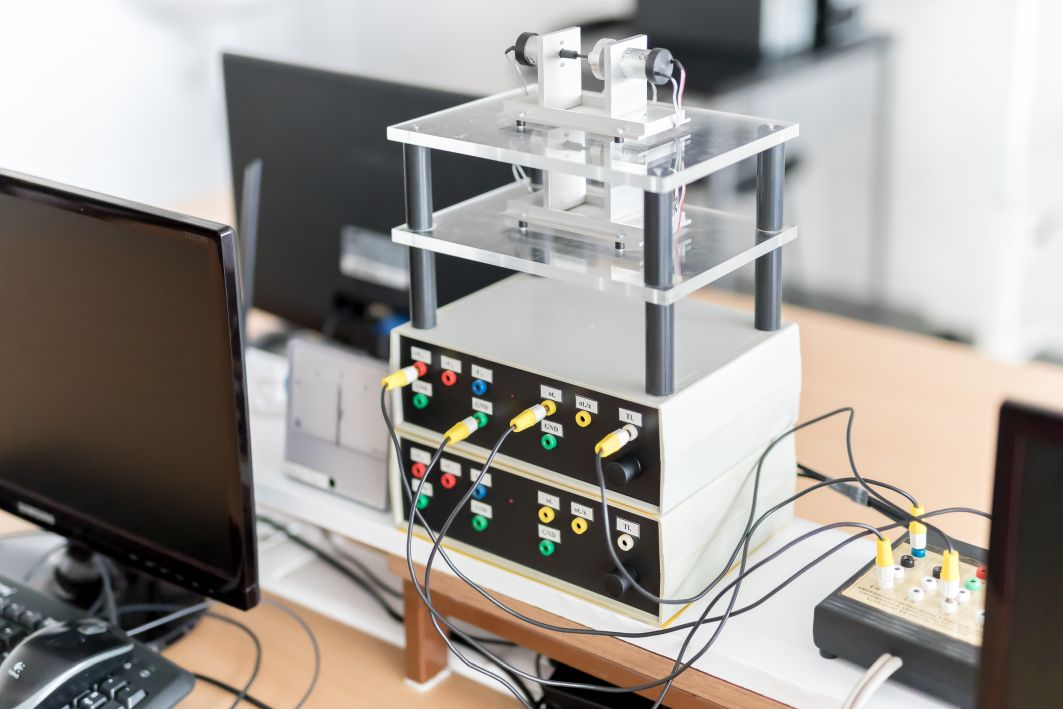
\includegraphics{IMG_6874_toPDF.jpg}
    }

    \figcaption{ 
        Celkový pohľad na laboratórne zariadenie LMOT.
    }

    \vspace{12pt}

    \label{IMG_6874_toPDF}
}%vbox
\end{figure}




% \begin{center}
    \begin{figure}[!t]

    \vbox{%
        \makebox[\textwidth][c]{%
        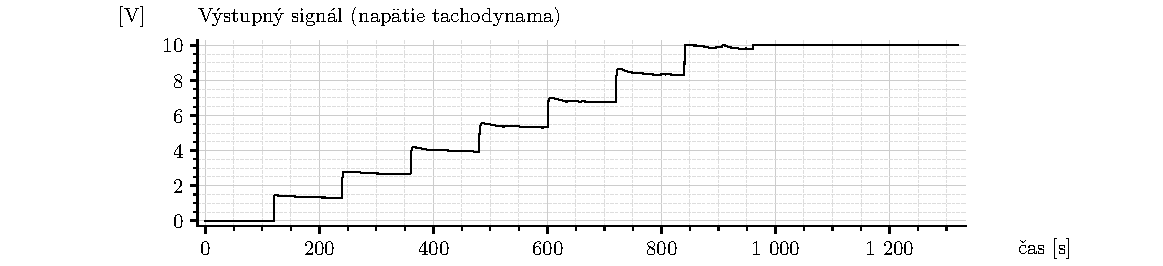
\includegraphics{fj_01_data_pot0_panel_1.pdf}
        }

        \makebox[\textwidth][c]{%
        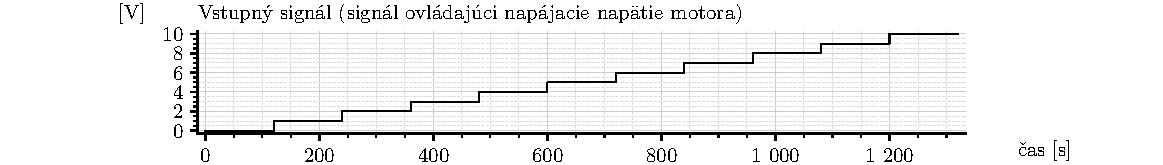
\includegraphics{fj_01_data_pot0_panel_3.pdf}
        }

        \makebox[\textwidth][c]{%
        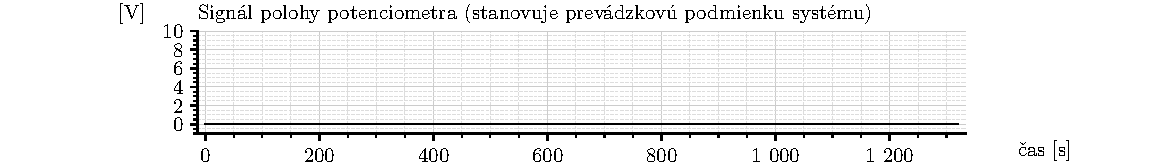
\includegraphics{fj_01_data_pot0_panel_2.pdf}
        }

        \figcaption{ 
        % \caption{
            Získané dáta pre vstupný signál a výstupný signál systému LMOT pri manuálne nastavenej prevádzkovej podmienke $0$ [V].
        }
        \label{fj_01_data_pot0}
    }%vbox

    \end{figure}
% \end{center}

\subsection{Získanie dát}


Empirické skúsenosti so systémom ukazujú, že výstup systému sa ustáli vždy ak sú vstupy systému ustálené. Pre vyšetrovanie ustálených stavov je teda možné využiť celý rozsah vstupného signálu a celý rozsah prevádzkových podmienok.




Pre získanie dát potrebných pre prevodovú charakteristiku sa uvažujú ustálené hodnoty vstupného signálu uvedené v tabuľke~\ref{tab:ustalene_hodnoty_vstupneho_signalu}.

\begin{center}

\vspace{-10pt}    
    
\tabcaption{Ustálené hodnoty vstupného signálu [V]}
\label{tab:ustalene_hodnoty_vstupneho_signalu}

\lstyle

\begin{tabular*}{\textwidth}{@{ \extracolsep{\fill}} ccccccccccc}
\toprule
0 & 1 & 2 & 3 & 4 & 5 & 6 & 7 & 8 & 9 & 10 \\
\bottomrule
\end{tabular*}

\end{center}





Napríklad je možné uvažovať prevádzkovú podmienku nastavenú na hodnotu $0$ [V]. Potom ak sa bude postupne meniť vstupný signál z~$0$ [V] na $10$ [V] a po každej zmene sa bude čakať na ustálenie výstupného signálu, je možné získať dáta pre prevodovú charakteristiku. Orientačné pozorovanie dynamiky systému ukazuje, že z praktického hľadiska sa systém ustáli do $15$ sekúnd po zmene na vstupe systému. Pre istotu, že výstup systému sa principiálne spoľahlivo ustáli je možné napríklad uvažovať čas $120$ sekúnd. Takto získané dáta sú zobrazené na obrázku~\ref{fj_01_data_pot0}.








\subsection{Spracovanie dát, nameraná prevodová charakteristika}


Zo získaných dát na obrázku \ref{fj_01_data_pot0} je potrebné vyňať úseky, počas ktorých sú výstupný a~vstupný signál ustálené. V tomto prípade nech za ustálený stav sa považuje posledných 30 \% zvoleného časového intervalu pre ustálenie, teda posledných 36 sekúnd z celkových 120 sekúnd. Takto vyňaté úseky sú znázornené na obrázku \ref{fj_02_data_pot0}.


% \begin{center}
    \begin{figure}[!b]

    \vbox{%
        \makebox[\textwidth][c]{%
        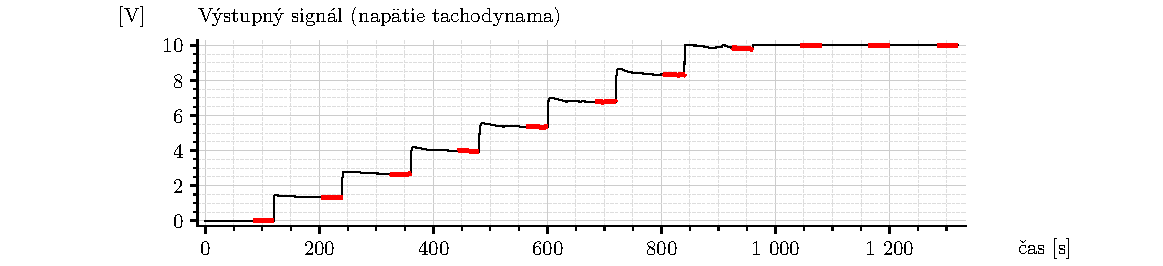
\includegraphics{fj_02_data_pot0_panel_1.pdf}
        }

        \makebox[\textwidth][c]{%
        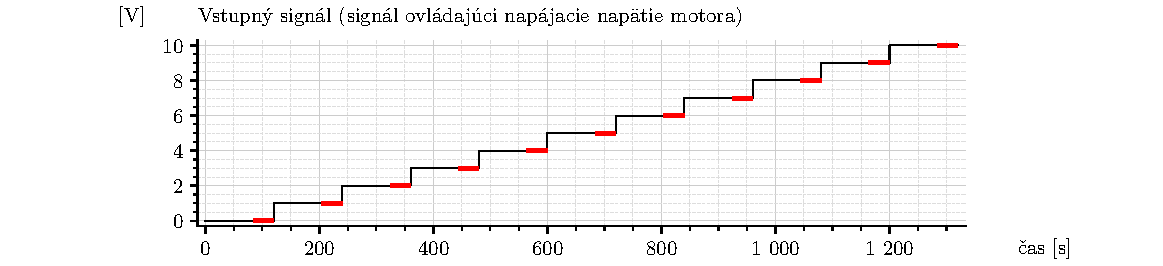
\includegraphics{fj_02_data_pot0_panel_3.pdf}
        }

        \vspace{-6pt}

        % \figcaption{ 
        \caption{
            % 
        }
        \label{fj_02_data_pot0}
    }%vbox

\end{figure}
% \end{center}

Pre všetky vyňaté úseky platí, že je možné vytvoriť dvojice hodnôt v zmysle ustálená hodnota vstupu k ustálenej hodnote výstupu. Grafické znázornenie uvedených dvojíc tak, že na x-ovej osi sú hodnoty vstupného signálu v ustálenom stave a na y-ovej osi sú prislúchajúce hodnoty výstupného signálu v~ustálenom stave, je vlastne grafickým vyjadrením nameranej prevodovej charakteristiky. Nameraná prevodová charakteristika je znázornená na obrázku \ref{fj_03_data_pot0_panel_1}.



% \begin{center}
    \begin{figure}[!t]

    \vbox{%
        \makebox[\textwidth][c]{%
        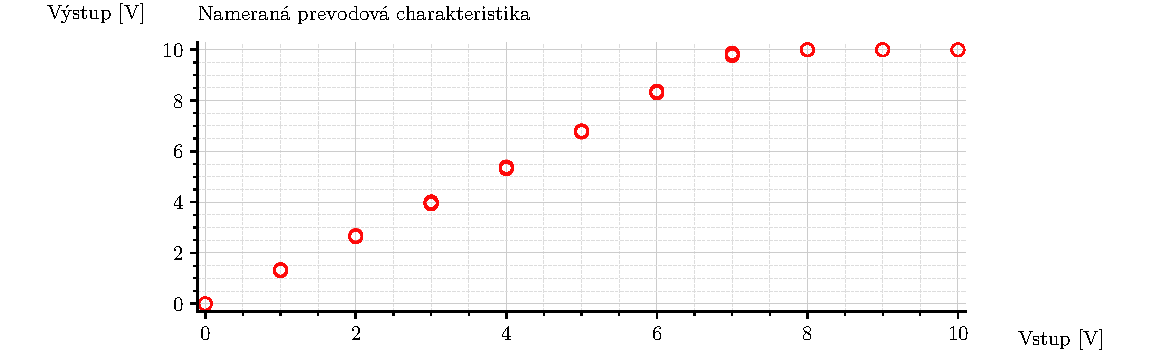
\includegraphics{fj_03_data_pot0_panel_1.pdf}
        }

        \vspace{-10pt}

        % \figcaption{ 
        \caption{
            Nameraná prevodová charakteristika pre prevádzkovú podmienku $0$ [V]. 
        }
        \label{fj_03_data_pot0_panel_1}
    }%vbox

\end{figure}
% \end{center}

% \begin{center}
    \begin{figure}[!b]

    \vbox{%
        \makebox[\textwidth][c]{%
        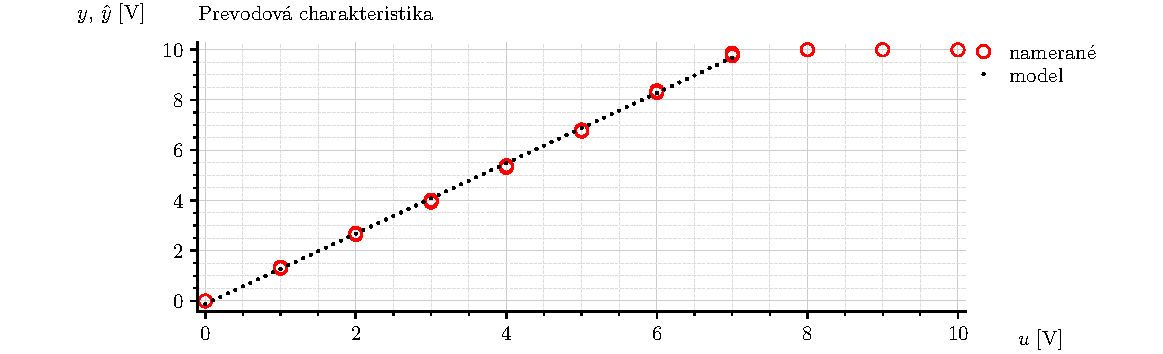
\includegraphics{fj_04_data_pot0_panel_1.pdf}
        }

        \vspace{-10pt}

        \figcaption{ 
        % \caption{
            % 
        }
        \label{fj_04_data_pot0_panel_1}
    }%vbox

\end{figure}
% \end{center}



\subsection{Aproximácia prevodovej charakteristiky}

Vstupnú veličinu označme ako $u$ a výstupnú veličinu ako $y$. Závislosť výstupnej veličiny od vstupnej veličiny potom je 
\begin{equation}
    y = f(u)
\end{equation}
kde $f$ je funkcia, ktorá vyjadruje aproximáciu prevodovej charakteristiky systému -- jej matematický model.

Z obrázku \ref{fj_03_data_pot0_panel_1} je zrejmé, že od hodnoty vstupného signálu $7$ [V] a viac je výstupná hodnota saturovaná na maxime (v podstate $10$ [V]). 

Na úseku $0 \leq u \leq 7$ [V], je možné usúdiť, že hľadaná závislosť je blízka priamke. Preto nech funkcia $f$ je daná polynómom prvého stupňa, teda
\begin{equation}
    f(u) = \Theta_1 u + \Theta_0
\end{equation}
kde $\Theta_1$ a $\Theta_0$ sú parametre, ktoré je potrebné určiť.

Parametre je možné určiť metódou najmenších štvorcov, čo v tomto prípade znamená minimalizovať sumu štvorcov odchýlok medzi nameranými hodnotami výstupného signálu a hodnotami vypočítanými z modelu. Formálne je odchýlka $ e = y - \hat y$. Takúto polynomiálnu aproximáciu bežne implementujú knižnice pre numerické výpočty pod názvom \texttt{polyfit}. Výsledkom (podrobnejší postup je nad rámec tohto textu) je 
\begin{equation}
    f(u) = 1,399\ u - 0,1196
\end{equation}
a táto funkcia (model prevodovej charakteristiky) je znázornená na obrázku \ref{fj_04_data_pot0_panel_1}.







\section{O prevodovej charakteristike zariadenia TS}

\subsection{Opis zariadenia}

TS, skratka od \emph{tepelný systém} (thermal system), je laboratórne zariadenie predstavujúce reálny dynamický systém. Tvorí ho sklenená trubica s ventilátorom a výhrevným telesom, pričom teplota vzduchu sa meria dvoma teplotnými snímačmi umiestnenými za výhrevným telesom a na opačnom konci trubice. Podstava obsahuje elektroniku zabezpečujúcu napájanie a rozhranie k meracej karte.

Fotografia laboratórneho zariadenia TS je na obrázku~\ref{TS_sch3_foto}.

Zariadenie má dva analógové vstupy a dva výstupy. Vstupy riadia výkon výhrevného telesa a ventilátora, zatiaľ čo výstupy predstavujú teplotu vzduchu v dvoch miestach trubice.

Z kybernetického hľadiska môže byť TS prevádzkovaný ako MIMO alebo SISO systém. Pri SISO konfigurácii je vstupom výkon výhrevného telesa a výkon ventilátora predstavuje prevádzkovú podmienku, keďže prúdenie vzduchu ovplyvňuje ohrievanie a~výslednú teplotu vzduchu.





\begin{figure}[!t]
% \begin{center}

    \vbox{%


        \makebox[\textwidth][c]{%
        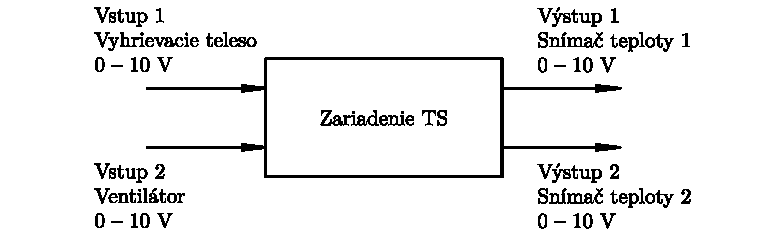
\includegraphics{TS_sch1.pdf}
        }

        \figcaption{ 
            Signály systému TS.
        }
        \label{TS_sch1}
    }%vbox

% \end{center}
\end{figure}


\begin{figure}[!b]
% \begin{center}

\vbox{%

    \makebox[\textwidth][c]{%
    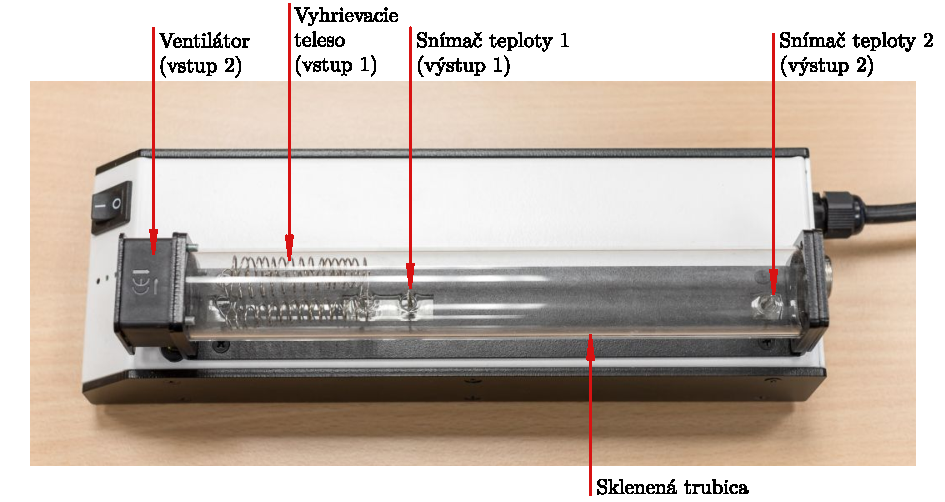
\includegraphics{TS_sch3_foto.pdf}
    }

    \figcaption{ 
        Pohľad zhora s vyznačením jednotlivých komponentov. 
    }
    \label{TS_sch3_foto}
}%vbox

% \end{center}
\end{figure}


V nasledujúcom sa uvažuje, že vstupným signálom je ten, ktorý ovláda ohrev špirály (Vstup~1). Prevádzková podmienka systému je realizovaná ventilátorom (Vstup~2).

Systém má dva výstupy – signály zo senzora 1 a senzora 2. Všetky signály (vstupný, výstupné aj signál prevádzkovej podmienky) nadobúdajú hodnoty v rozsahu $0$ až $10$ pričom ide o napäťové signály vo voltoch [V].



\begin{center}

\vspace{-10pt}    
    
\tabcaption{Rozsahy a jednotky signálov}
\label{tab:rozsahy_a_jednotky_signalu}

\lstyle

\begin{tabular*}{\textwidth}{@{ \extracolsep{\fill}} lll}
\toprule
Signál & Rozsah hodnôt & Jednotka \\
\midrule
Vstup 1 & $0$ až $10$ & V (volt) \\
Vstup 2 & $0$ až $10$ & V (volt) \\
Výstup 1 & $0$ až $10$ & V (volt) \\
Výstup 2 & $0$ až $10$ & V (volt) \\
\bottomrule
\end{tabular*}


\end{center}




\subsection{Získanie dát}

Empirické skúsenosti so systémom ukazujú, že výstupy systému sa ustália vždy, ak sú vstupný signál a prevádzková podmienka ustálené.

Meranie uvažuje ustálené hodnoty vstupného signálu uvedené v~tabuľke~\ref{tab:ustalene_hodnoty_vstupneho_signalu} a~napríklad hodnotu prevádzkovej podmienky $6$ [V].

\begin{center}

\vspace{-10pt}    
    
\tabcaption{Ustálené hodnoty vstupného signálu [V]}
\label{tab:ustalene_hodnoty_vstupneho_signalu}

\lstyle

\begin{tabular*}{\textwidth}{@{ \extracolsep{\fill}} ccccccccccc}
\toprule
0 & 1 & 2 & 3 & 4 & 5 & 6 & 7 & 8 & 9 & 10 \\
\bottomrule
\end{tabular*}

\end{center}

Predmetný systém  má relatívne pomalú dynamiku. Vo všeobecnosti sa systém dokáže úplne ustáliť približne do $1$ až $3$ minút po zmene vstupného signálu, avšak v niektorých prípadoch nemusí byť ani čas $10$ minút postačujúci na úplné ustálenie. Zvolený bol čas ustálenia $5$ minút pre ustálené hodnoty vstupného signálu $1$ až $10$ [V]. Pre nulovú hodnotu vstupného signálu bol z dôvodu pomalšieho poklesu teploty zvolený čas ustálenia $10$ minút.

\begin{figure}[!t]

\vbox{%
    \makebox[\textwidth][c]{%
    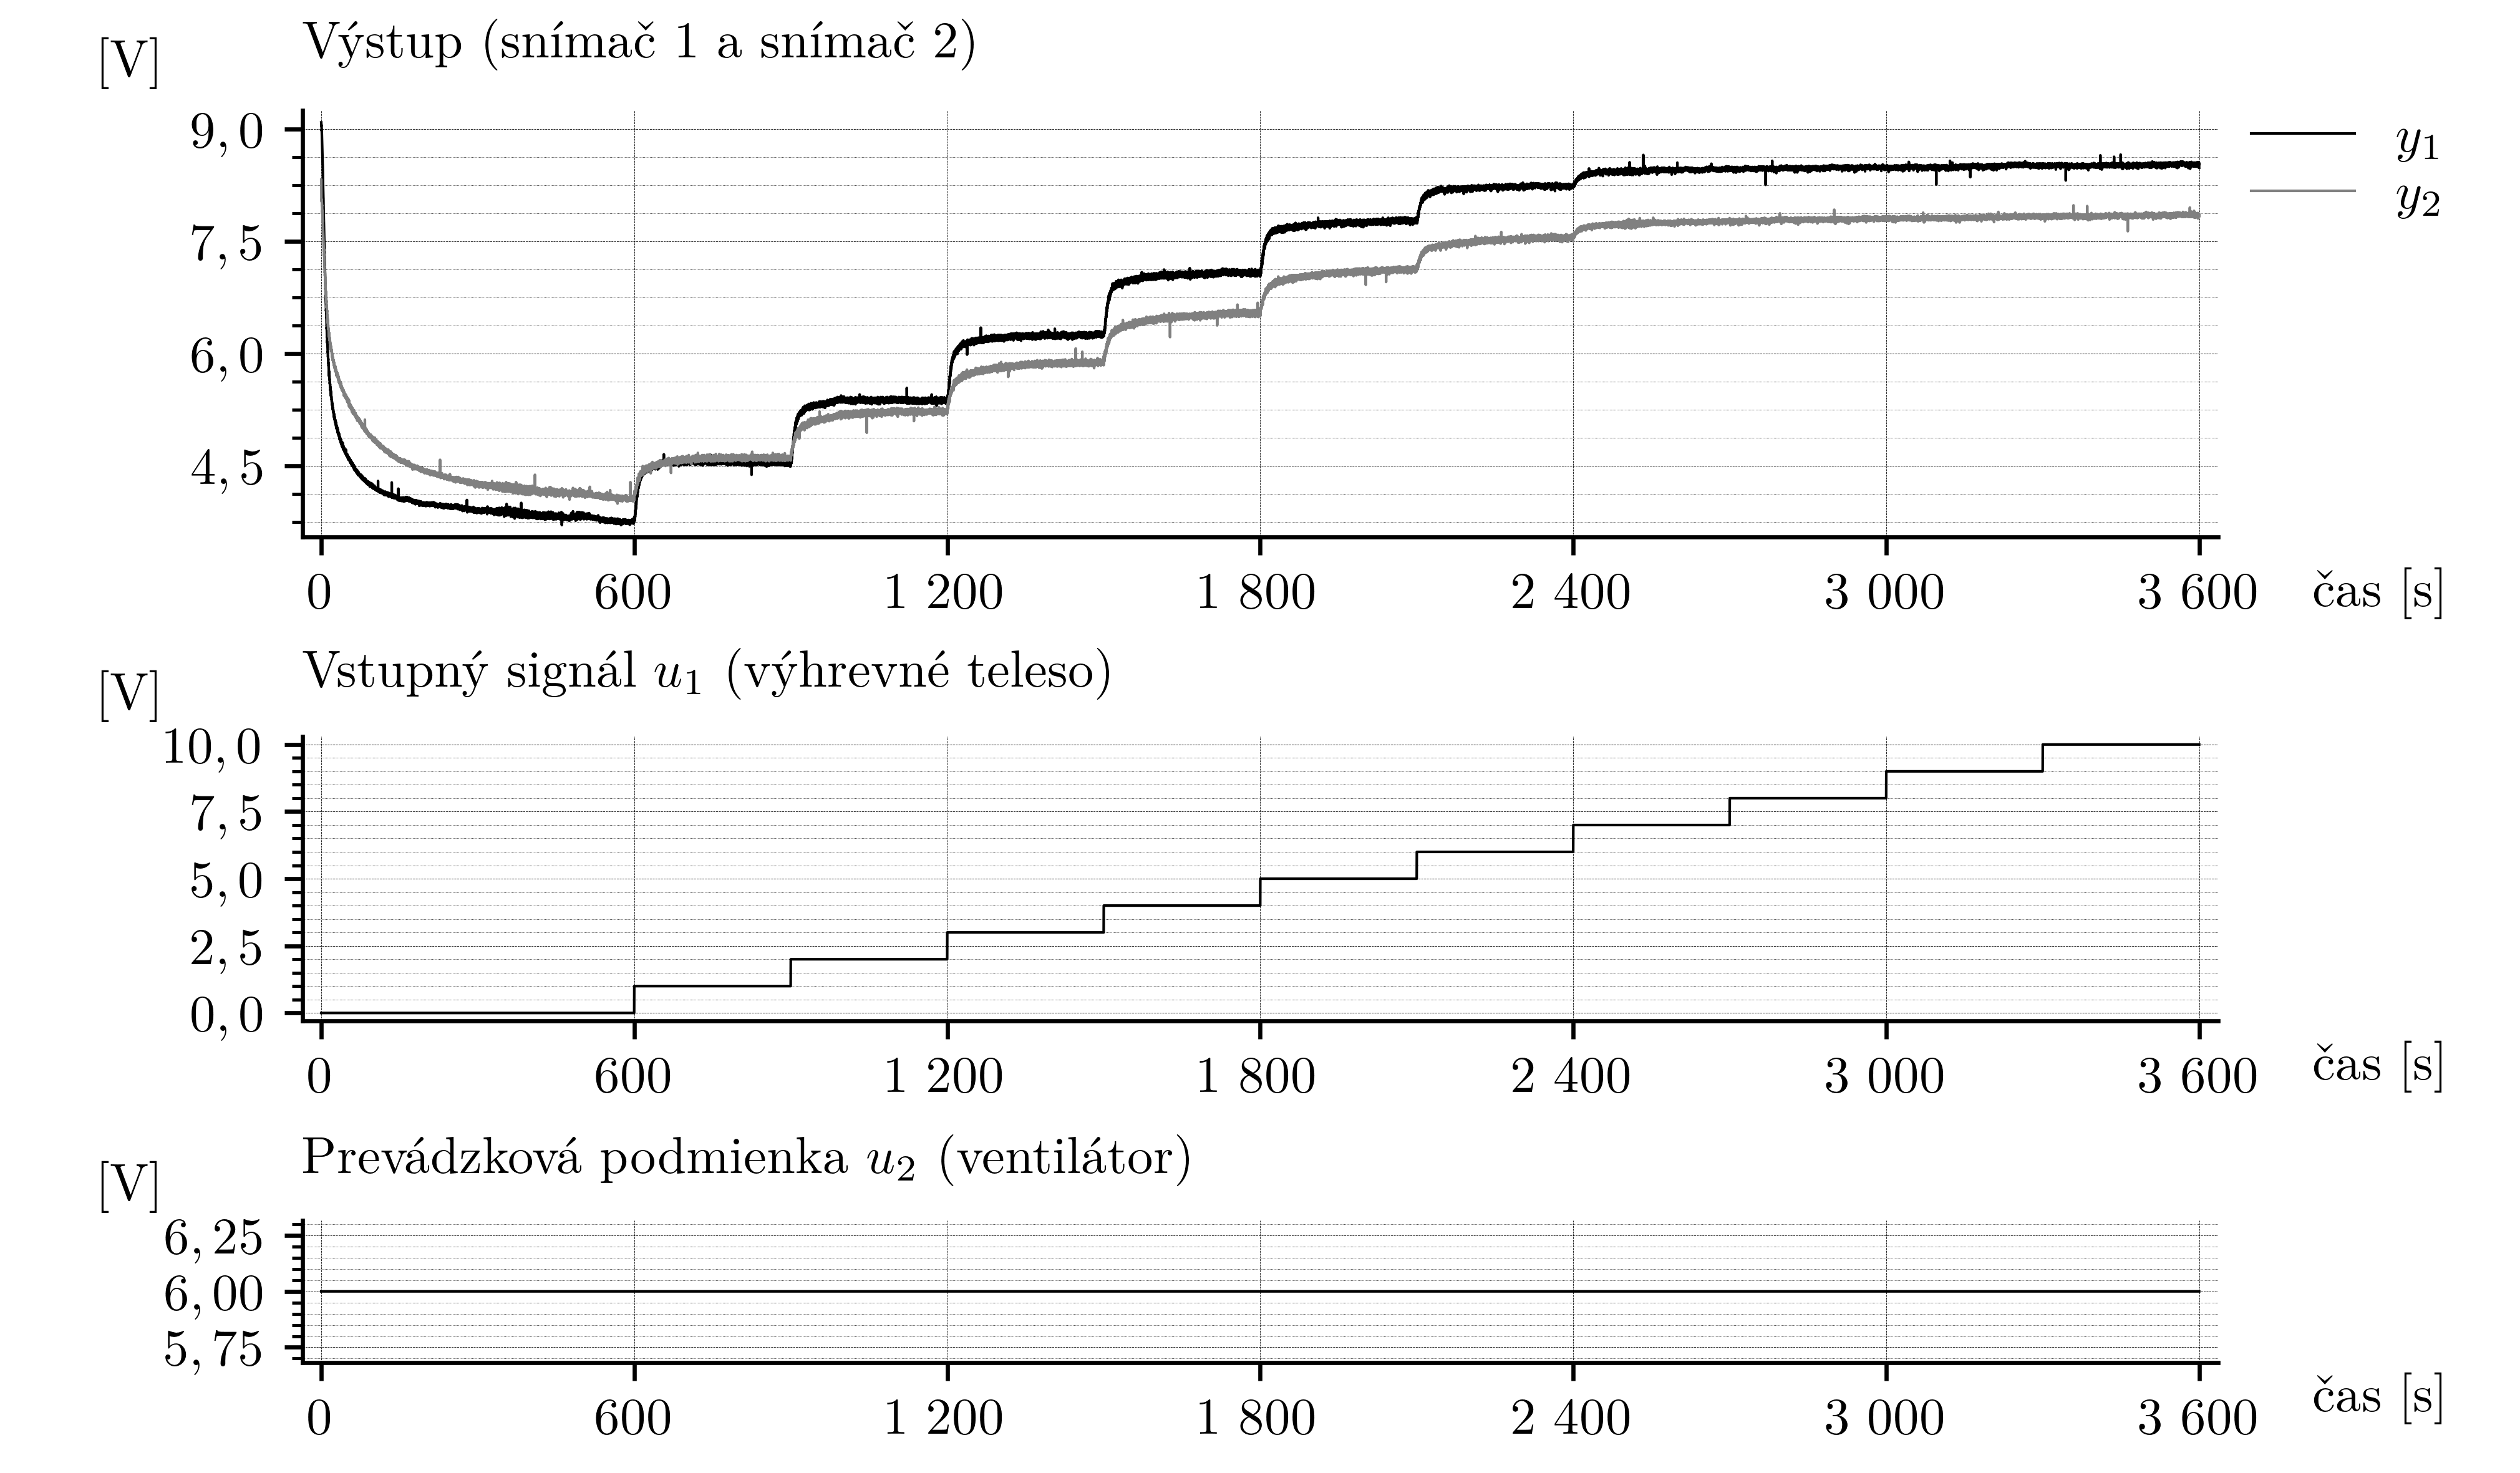
\includegraphics{exp3_meranie.png}
    }

    \figcaption{
        Získané dáta pre vstupný signál a výstupné signály systému TS pri manuálne nastavenej prevádzkovej podmienke ventilátora $6$~[V].
    }
    \label{fj_01_data_ts_pot6}
}%vbox

\end{figure}



\subsection{Spracovanie dát, nameraná prevodová charakteristika}

\begin{figure}[!t]

\vbox{%
    \makebox[\textwidth][c]{%
    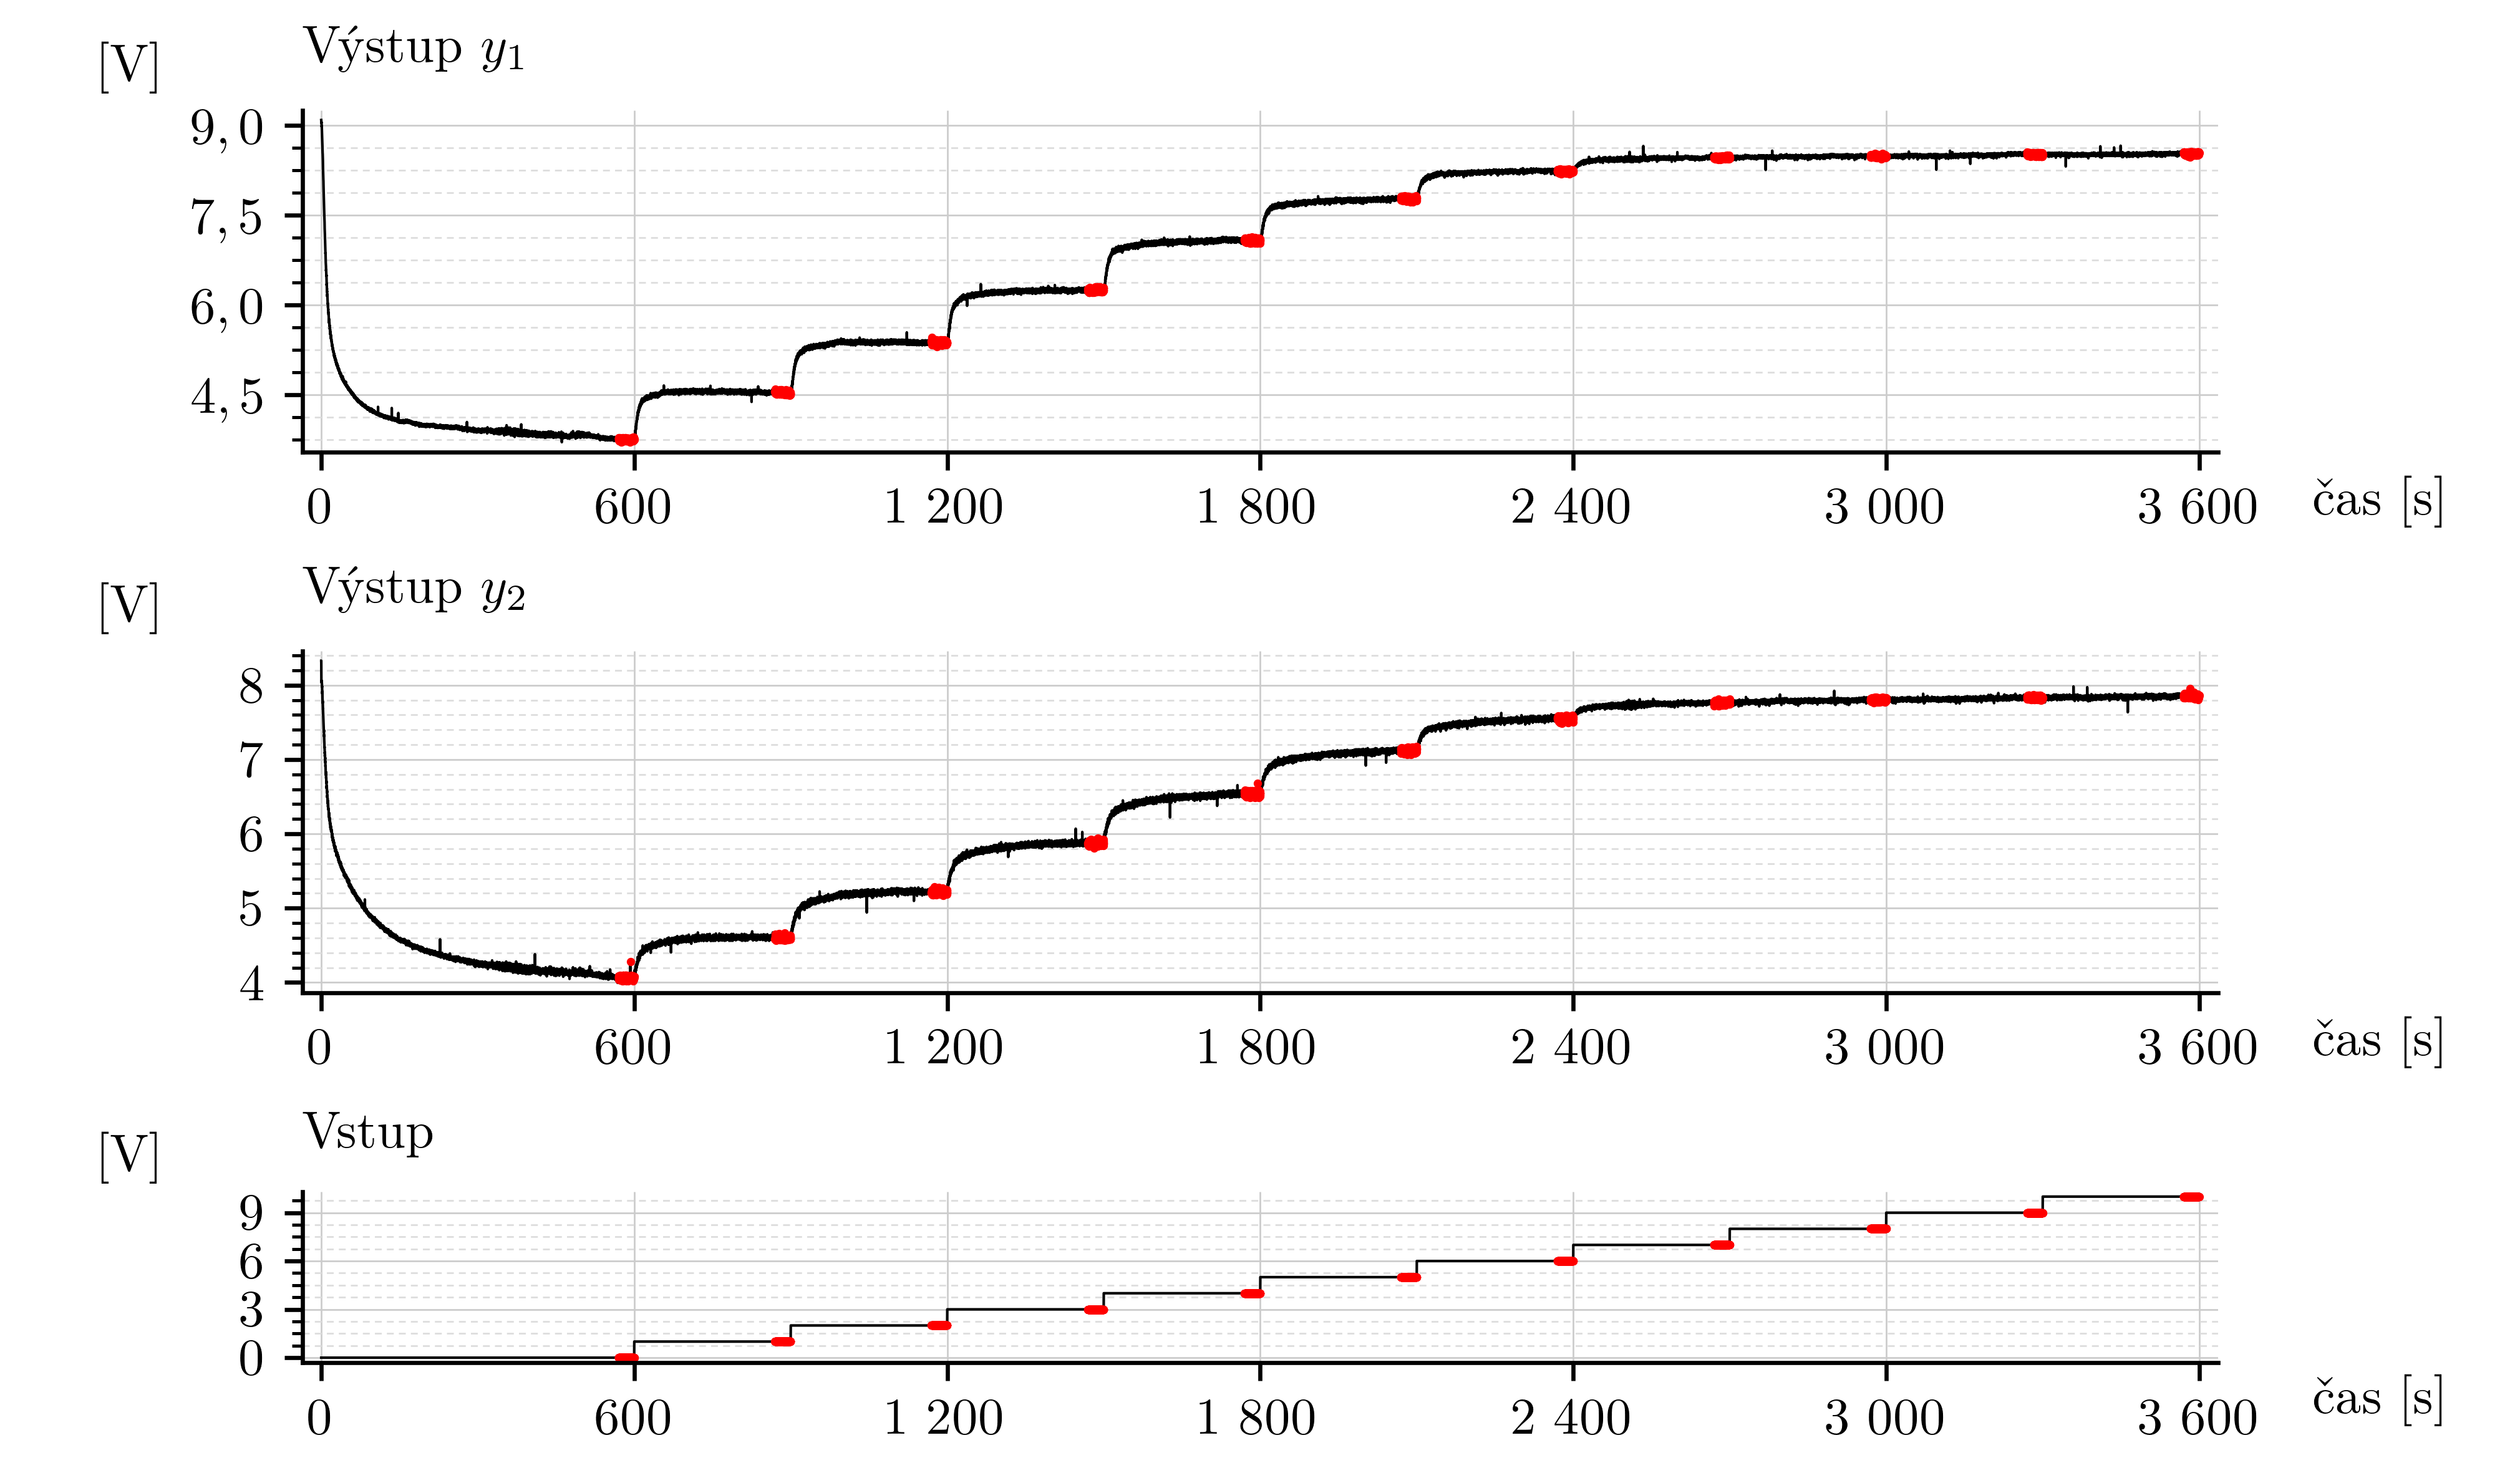
\includegraphics{exp3_meranie_steadyPoints.png}
    }

    \vspace{-6pt}

    \caption{
        %
    }
    \label{fj_02_data_ts_pot6}
}%vbox

\vspace{-10pt}

\end{figure}

Zo získaných dát na obrázku \ref{fj_01_data_ts_pot6} je potrebné vyňať úseky, počas ktorých sú výstupné a~vstupné signály ustálené. V tomto prípade nech za ustálený stav sa považuje posledných $30$ sekúnd zvoleného časového intervalu pre ustálenie, pričom posledných $0.1$ sekundy merania sa neuvažuje. Takto vyňaté úseky sú znázornené na obrázku \ref{fj_02_data_ts_pot6}.

Pre všetky vyňaté úseky platí, že je možné vytvoriť dvojice hodnôt v zmysle ustálená hodnota vstupu k ustálenej hodnote výstupu. Grafické znázornenie uvedených dvojíc tak, že na x-ovej osi sú hodnoty vstupného signálu v ustálenom stave a na y-ovej osi sú prislúchajúce hodnoty výstupného signálu v~ustálenom stave, je vlastne grafickým vyjadrením nameranej prevodovej charakteristiky. Nameraná prevodová charakteristika je znázornená na obrázku~\ref{fj_03_data_ts_panel_1}. 

% \begin{center}
\begin{figure}[!b]

\vspace{-12pt}

\vbox{%
    \makebox[\textwidth][c]{%
    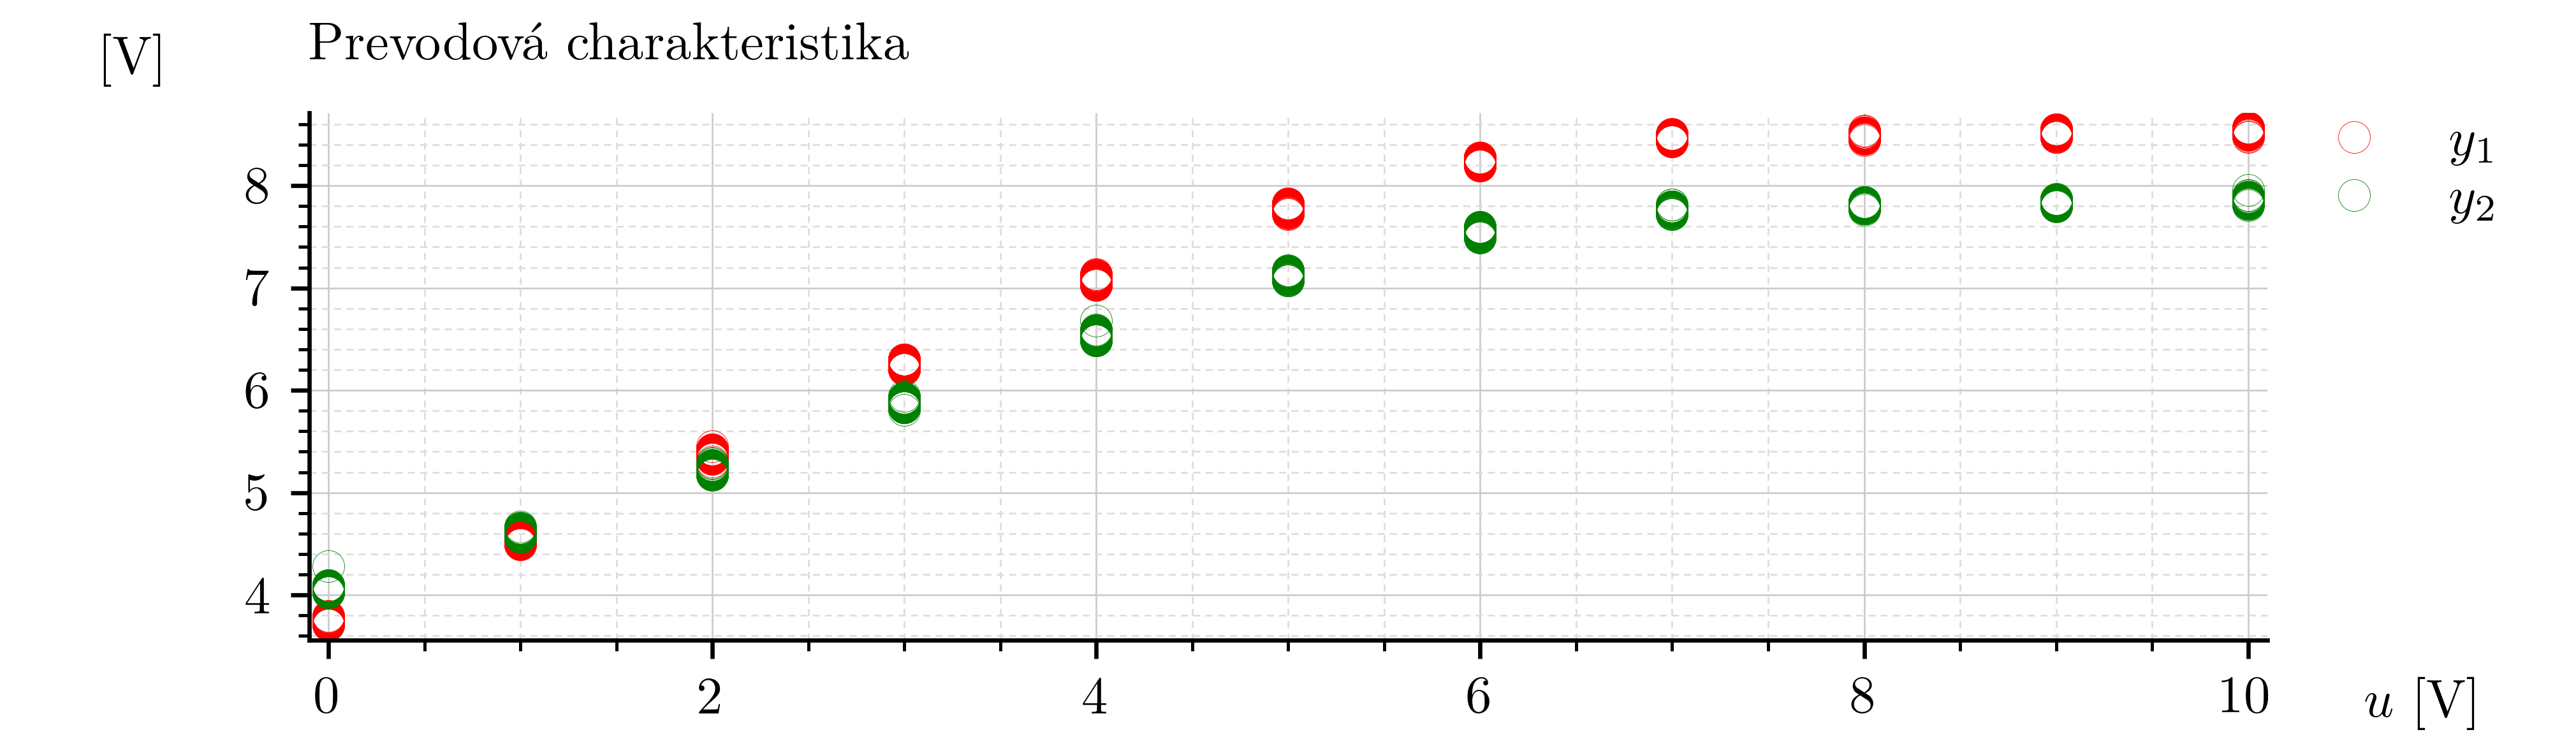
\includegraphics{exp3_prevodova.png}
    }

    \vspace{-6pt}

    \caption{
        Nameraná prevodová charakteristika systému TS pre prevádzkovú podmienku $6$ [V].
    }
    \label{fj_03_data_ts_panel_1}
}%vbox

\vspace{-10pt}

\end{figure}
% \end{center}


\subsection{Aproximácia prevodovej charakteristiky}

Ukazuje sa, že pre hodnoty vstupného signálu približne od $7$~[V] dochádza k saturovaniu výstupných veličín. Z tohto dôvodu je účelné rozdeliť prevodovú charakteristiku na dve časti.

Vstupnú veličinu označme ako $u$. Závislosť výstupných veličín od vstupnej veličiny potom je
\begin{equation}
y_1 = f_1(u), \qquad y_2 = f_2(u)
\end{equation}

Na úseku $0 \leq u \leq 7$~[V] je možné na základe grafického zobrazenia nameraných dát aproximovať závislosť lineárnou funkciou. Parametre lineárnej aproximácie boli určené metódou najmenších štvorcov pomocou funkcie \texttt{polyfit} (z adekvátnej softvérovej knižnice a adekvátnym postupom). Výsledkom sú modely
\begin{align}
y_1 &= 0,709533\,u + 3,951781 \\
y_2 &= 0,559831\,u + 4,135048
\end{align}

Pre hodnoty vstupného signálu $7 < u \leq 10$~[V] sú výstupné veličiny saturované. Priemerné hodnoty výstupov v tejto oblasti sú
\begin{align}
y_1 &= 8,500301 \\
y_2 &= 7,815181
\end{align}
Takto získaná aproximácia prevodovej charakteristiky je znázornená na obrázku~\ref{fj_04_data_ts_panel_1}.



\begin{figure}[!t]

\vbox{%
    \makebox[\textwidth][c]{%
    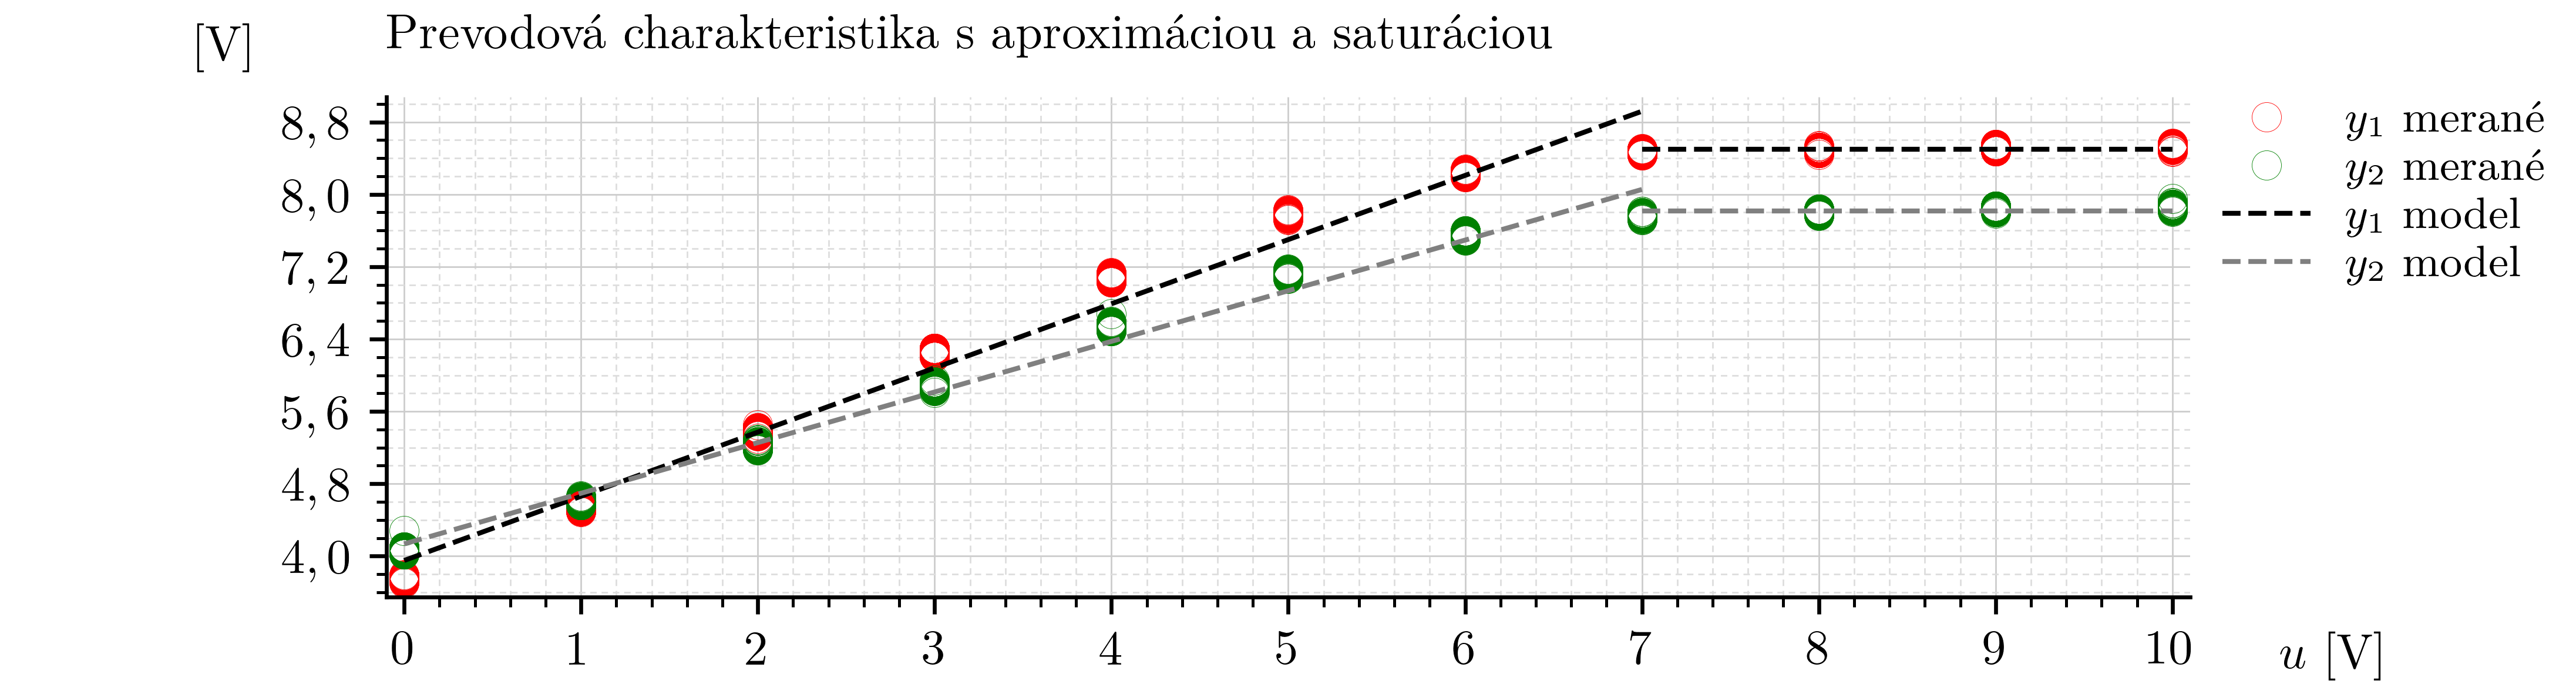
\includegraphics{exp3_prevodova_fit_sat.png}
    }

    \vspace{-6pt}

    \figcaption{
        Aproximácia nameranej prevodovej charakteristiky systému TS lineárnym modelom so saturovanou časťou.
    }
    \label{fj_04_data_ts_panel_1}
}%vbox

\end{figure}












\end{document}
